\documentclass[prd,twocolumn,amsmath,amssymb,floatfix,superscriptaddress,nofootinbib]{revtex4-1}
\usepackage{bm}
\usepackage{amsmath}
\usepackage{epsfig}
\usepackage{color}
\usepackage{natbib}
\usepackage{textcase}
\usepackage{graphicx}
\usepackage{ifthen}
\usepackage{xstring}
\usepackage{graphicx}
\usepackage[utf8]{inputenc} 
\usepackage{amssymb}
\usepackage{latexsym}
\usepackage{epstopdf}
\epstopdfsetup{update}
\DeclareGraphicsExtensions{.ps, .png}
\epstopdfDeclareGraphicsRule{.ps}{pdf}{.pdf}{ps2pdf -dEPSCrop -dNOSAFER #1 \OutputFile} 
\usepackage{dcolumn} 
\usepackage{multirow}
\usepackage{appendix}
\usepackage{footnote}
\usepackage{tabularx,ragged2e,booktabs}
\usepackage[normalem]{ulem}
\usepackage{float}
\restylefloat{table}

\newcommand{\Omegamzero}{\Omega_{{\rm m,0}}}
\newcommand{\Rbar}{$\bar{R}$}
\newcommand{\lsc}{\mathcal{L}}
\newcommand{\rhom}{\rho_{\rm m}}
\newcommand{\Mpch}{\mbox{Mpc}/h}
\newcommand{\iMpch}{h/\mbox{Mpc}}
\newcommand{\Msun}{M_\odot}
\newcommand{\Mv}{M_{\rm v}}

\newcommand{\refsec}[1]{section~\ref{sec:#1}}
\newcommand{\refeq}[1]{Eq.~(\ref{eq:#1})}
\newcommand{\refssec}[1]{section~\ref{subsec:#1}}
\newcommand{\reffig}[1]{Fig.~\ref{fig:#1}}
\newcommand{\refFig}[1]{Fig.~\ref{fig:#1}}
\newcommand{\curv}{{\cal R}}
\newcommand{\xef}{x_e^{\rm fid}}
\newcommand{\xmax}{x_e^{\rm max}}
\newcommand{\zmax}{z_{\rm max}}
\newcommand{\zmin}{z_{\rm min}}
\newcommand{\xemin}{x_e^{\rm min}}

\newcommand{\ra}{\rightarrow}
\def\max{_{\mathrm{max}}}
\def\lsim{\mathrel{\raise.3ex\hbox{$$<$$\kern-.75em\lower1ex\hbox{$\sim$}}}}
\def\gsim{\mathrel{\raise.3ex\hbox{$$>$$\kern-.75em\lower1ex\hbox{$\sim$}}}}

\newcommand{\beq}{\begin{equation}}
\newcommand{\eeq}{\end{equation}}

\newcommand{\bea}{\begin{eqnarray}}
\newcommand{\eea}{\end{eqnarray}}

\newcommand{\wh}[1]{\textcolor{blue}{#1}}
\newcommand{\ch}[1]{\textcolor{red}{#1}}

\def\mnras{Mon.\ Not.\ R.\ Astron.\ Soc.\ }
\definecolor{darkgreen}{cmyk}{0.85,0.2,1.00,0.2} 
\definecolor{purple}{cmyk}{0.5,1.0,0,0} 
\def\physrep{Phys.~Rep.}

\definecolor{ultramarine}{rgb}{0.07, 0.04, 0.56}
\definecolor{cadmiumgreen}{rgb}{0.0, 0.42, 0.24}
\definecolor{indigo(dye)}{rgb}{0.0, 0.25, 0.42}
\usepackage[linktocpage=true]{hyperref}
\hypersetup{
colorlinks=true,
citecolor=ultramarine,
linkcolor=cadmiumgreen,
urlcolor=indigo(dye),
pdfauthor={},
pdftitle={},
pdfsubject={}
}


\begin{document}
	
\title{Reionization Planck 2018 ...}

\author{Chen Heinrich}\email{chenhe@caltech.edu}
\affiliation{$Jet\ Propulsion\ Laboratory,\ California\ Institute\ of\ Technology,\ Pasadena,\ California\ 91109,\ USA$}
\affiliation{$California\ Institute\ of\ Technology,\ Pasadena,\ California\ 91109,\ USA$}

\author{Wayne Hu}
\affiliation{Kavli Institute for Cosmological Physics, Enrico Fermi Institute, University of Chicago, Chicago Illinois 60637}
\affiliation{Department of Astronomy \& Astrophysics,
 University of Chicago, Illinois 60637}

\begin{abstract}

...

\end{abstract}
\pacs{}

\maketitle

\section{Introduction}
\label{sec:intro}

Trying to collect all of our tests here.\\

List of tests:\\
\begin{itemize}
    \item {Direct MCMC chains
        \begin{enumerate}
            \item {PC zmax = 30}
            \item {PC zmax = 50}
            \item{tanh tau}
            \item{tanh highz model}
        \end{enumerate}
    }
    \item{best tests
        \begin{enumerate}
            \item {from tanh highz 2-parameter model we found that for tau hi > 0.02, we get ML is tau hi = 0.0206, tau lo = 0.0414 corresponding to zre = 6.29 and xe hi = 0.0748. This model has a -loglike = 499.5458 against the full ML 498.2425 which gives a difference of 2.6 in chi2. (full ML has tau lo = 0.0543, tau hi = 0.00542 corresponding to zre = 7.68 and xe hi = 0.0214. }
            \item{Using above informatiion, we fixed tau hi = 0.02, and ran a best-fit searching for best tau lo and found tau lo = 0.045 (c.f. 0.0414 from chains), together with the fixed tau hi = 0.02, corresponds to zre = 6.67 and xe min = 0.073. The likelihood here is 499.2914, a difference of 2.1 (instead of 2.6) in chi2.}
        \end{enumerate}
        }

    
    \item {Direct MCMC chains}
    
\end{itemize} 



\begin{figure}
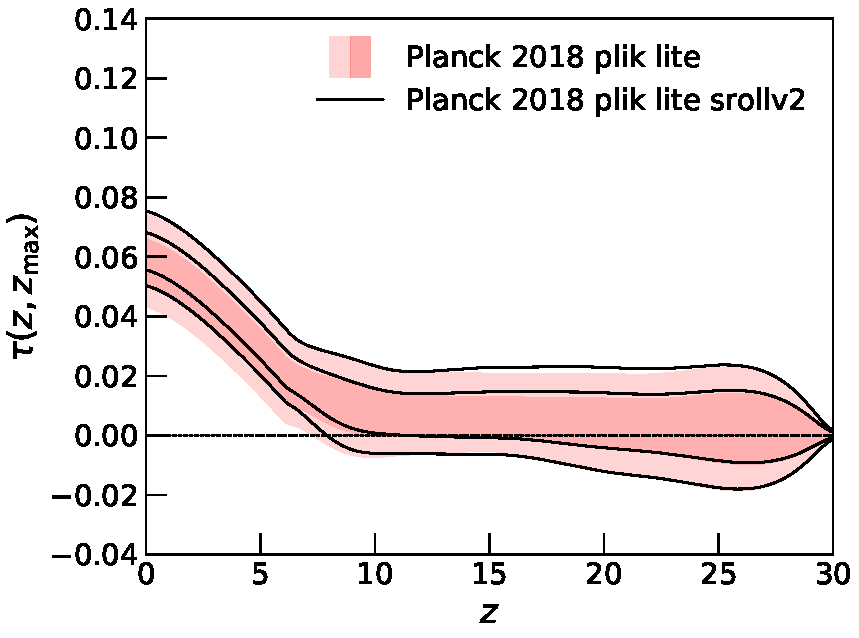
\includegraphics[width=0.40\textwidth]{results/cosmomc_runs/pl18_plots_zmax30/plot_pub_tau_gtz_dz_0p1_pl18_pc_zmax30_pliklite_post_0930_and_pl18_pc_zmax30_pliklite_srollv2_0930.pdf}
\caption{Comparing zmax = 50 PC chains using Planck 2018 original lowE vs srollv2 likelihood (plik\_lite\_TTTEEE + lowl + simall\_EE vs plik\_lite\_TTTEEE + lowl + sroll2\_EE).
}
\label{fig:}
\end{figure}

\begin{figure}
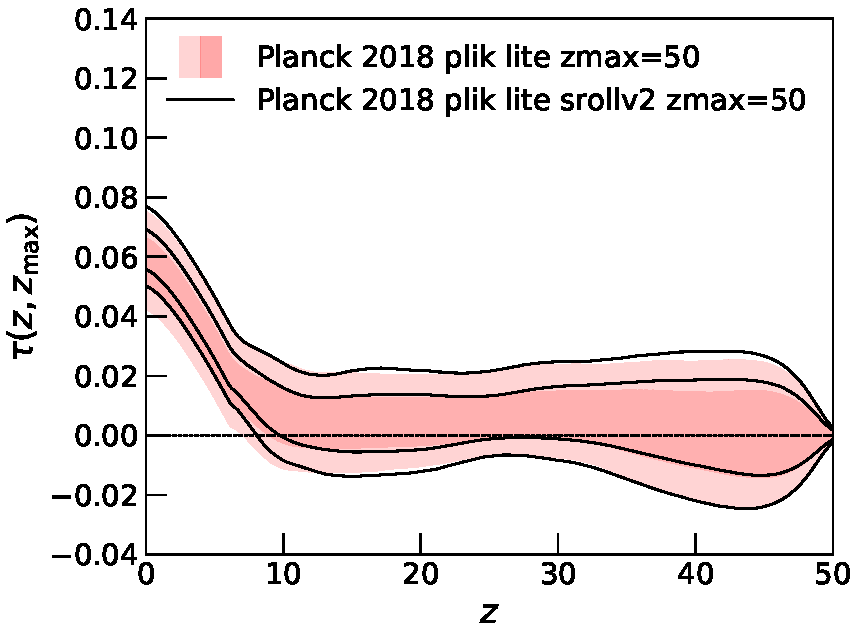
\includegraphics[width=0.40\textwidth]{results/cosmomc_runs/pl18_plots_zmax50/plot_pub_tau_gtz_dz_0p1_pl18_pc_zmax50_pliklite_post_and_pl18_pc_zmax50_pliklite_srollv2.pdf}
\caption{Comparing zmax = 50 PC chains using Planck 2018 original lowE vs srollv2 likelihood (plik\_lite\_TTTEEE + lowl + simall\_EE vs plik\_lite\_TTTEEE + lowl + sroll2\_EE).
}
\label{fig:}
\end{figure}


\begin{figure}
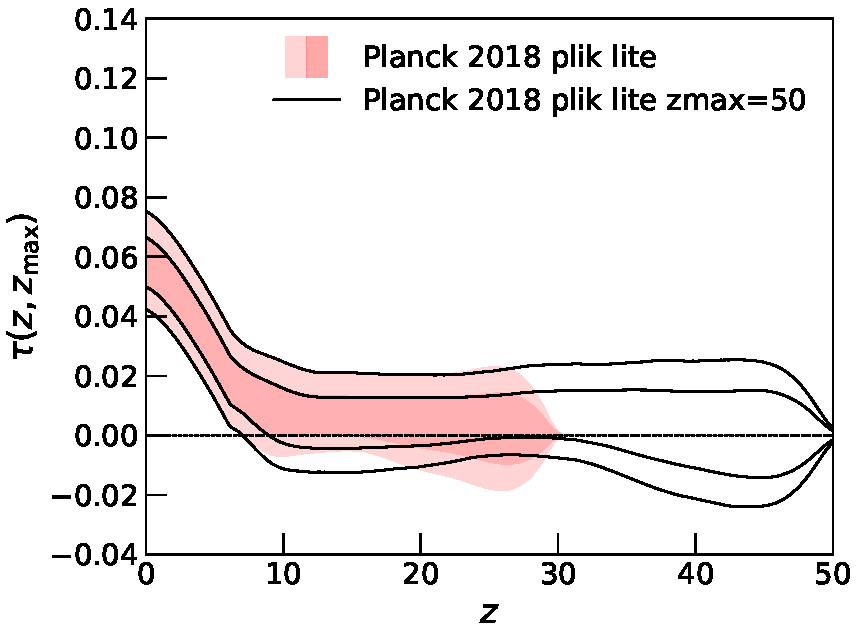
\includegraphics[width=0.40\textwidth]{results/cosmomc_runs/pl18_plots_zmax30/plot_pub_tau_gtz_dz_0p1_pl18_pc_zmax30_pliklite_post_0930_and_pl18_pc_zmax50_pliklite_post.pdf}
\caption{Comparing zmax = 30 and 50 PC chains using Planck 2018 original lowE likelihood (plik\_lite\_TTTEEE + lowl + simall\_EE). Note that the zmax = 30 uses 5 PCs, whereas the zmax = 50 chains uses 7 PCs.
}
\label{fig:tau_gtz_zmax_30_vs_50_simall_EE}
\end{figure}


\begin{figure}
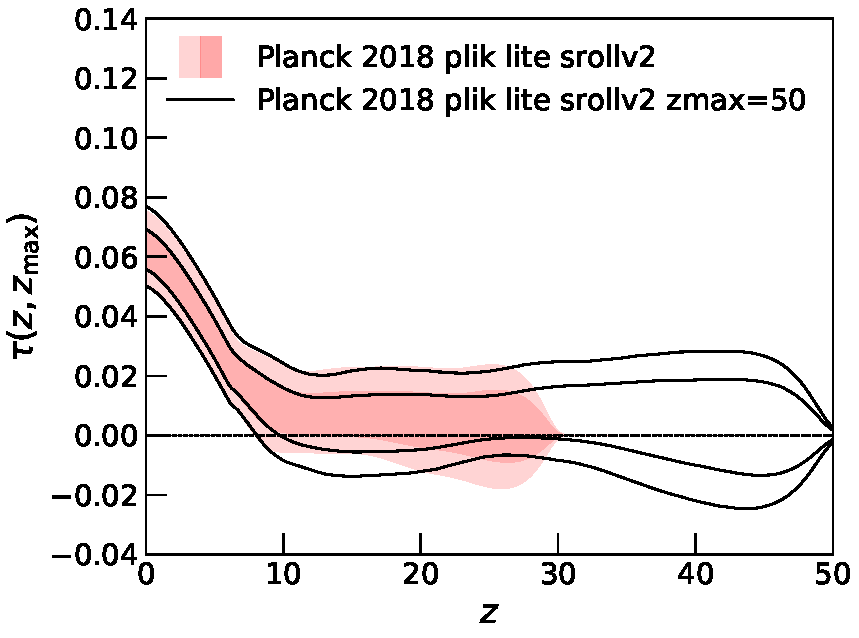
\includegraphics[width=0.40\textwidth]{results/cosmomc_runs/pl18_plots_zmax30/plot_pub_tau_gtz_dz_0p1_pl18_pc_zmax30_pliklite_srollv2_0930_and_pl18_pc_zmax50_pliklite_srollv2.pdf}
\caption{Same as Fig.~\ref{fig:tau_gtz_zmax_30_vs_50_simall_EE}, but for the srollv2 likelihood (plik\_lite\_TTTEEE + lowl + sroll2\_EE).
}
\label{fig:}
\end{figure}

\begin{figure}[t]
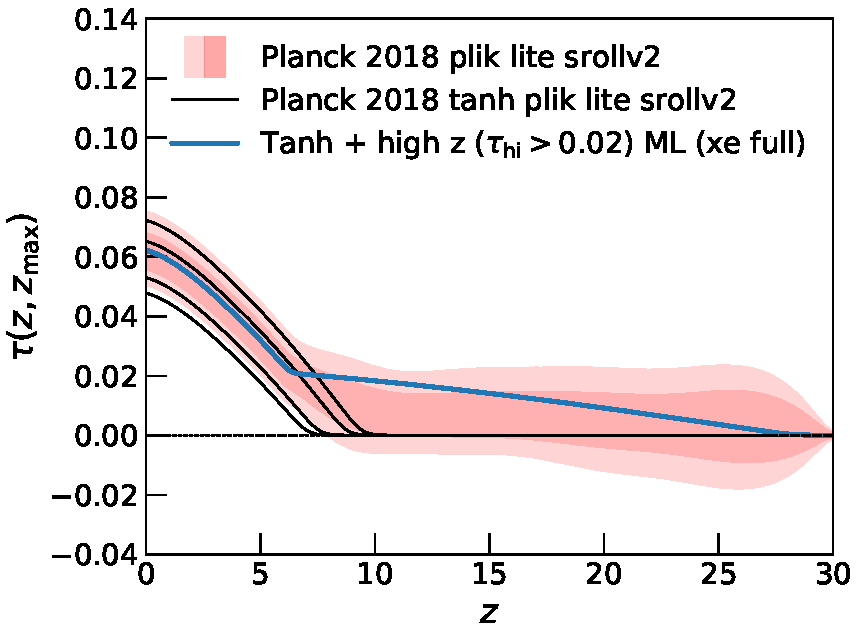
\includegraphics[width=0.40\textwidth]{../paper/plots/plot_tau_gtz.pdf}
\caption{...
}
\label{fig:}
\end{figure}


\begin{figure}
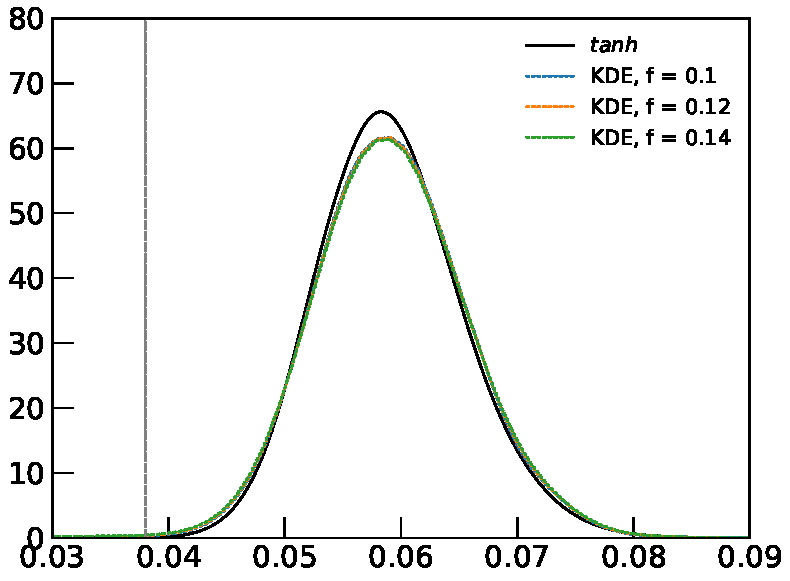
\includegraphics[width=0.40\textwidth]{python_kde_test/pl18_pc_zmax30_pliklite_srollv2_1015_tau_posterior_fraccov_1p0_burnin_10000_yes_norm_gaussian0p1_0p12_0p14.pdf}
\caption{...
}
\label{fig:}
\end{figure}

\bibliography{rei.bib}

\end{document}
